% --------------------------------------------------------------
% Abhi's Standard Preamble.
% --------------------------------------------------------------
 
\documentclass[12pt]{article}
 
%Packages
\usepackage[margin=1in]{geometry} 
\usepackage{graphicx}
\usepackage{url}
\usepackage{hyperref}
\usepackage{float}
\usepackage{quoting}

\usepackage{aurical}
 
\begin{document}
 
\title{Opi Fex Veneficiorum}
\date{}

\maketitle

\begin{figure}[H]
  \centering
  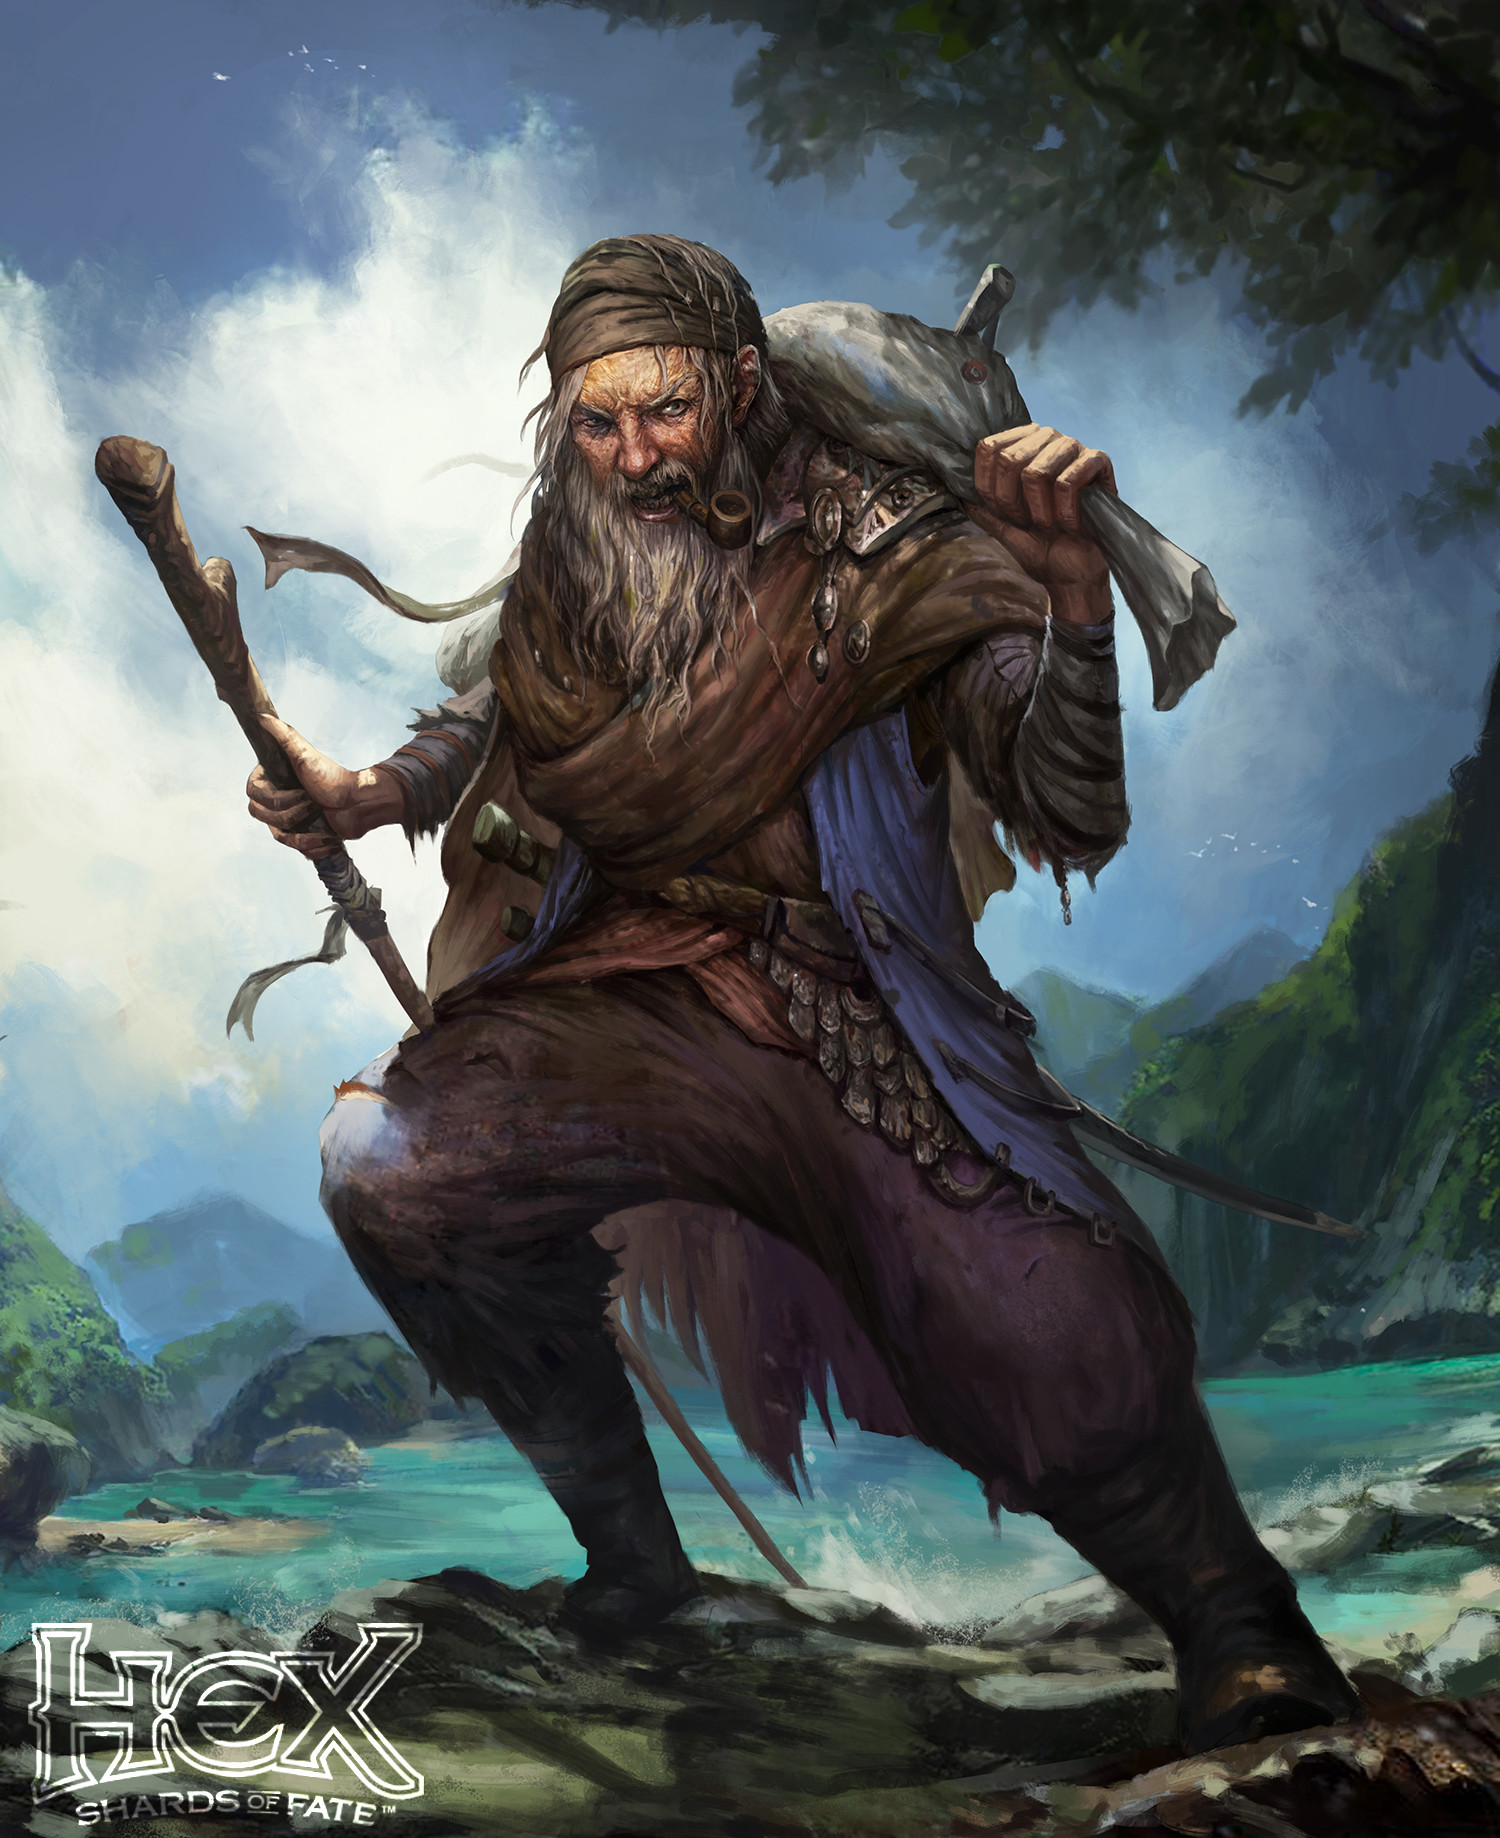
\includegraphics[width=.8125\textwidth]{./resources/OpiFexVeneficiorum}
  \caption{
    Opi. Once a worldly village blacksmith, now far more driven. {\bf Note:} his name, written as
    {\it Opifex Veneficiorum} means "Smith of Spells" in Latin.
  }
\end{figure}

\section{Character Description}

Although vague attempts have been made to tame it with a bandana, dirty grey hair litters the face
of Opi Fex Veneficiorum. Opi changes attire rather often, usually due to experimentation rendering
the previous set, {\it ahem}, without the ability to function as clothing. For similar reasons his
current weapon (walking stick?) of choice is merely a glorified branch. However, should one look
closely, a small arcane script can be found inscribed in various corners of all of his possessions,
catalysts for various incantations. Opi maintains a steady and cautious personality to his
acquaintances, but those who know him bettter recognize his propensity to flights of fancy and
obsession to his craft. 

His only pieces of luxury adornments are his pipe, which he can be frequently found smoking or
otherwise fiddling with, and a plain locket around his neck. The locket opens up to reveal
a portrait of woman, his lover {\it Favilla}. He rarely speaks more than one or two words about her,
but his eyes betray his affection, and sorrow.

\begin{figure}[H]
  \centering
  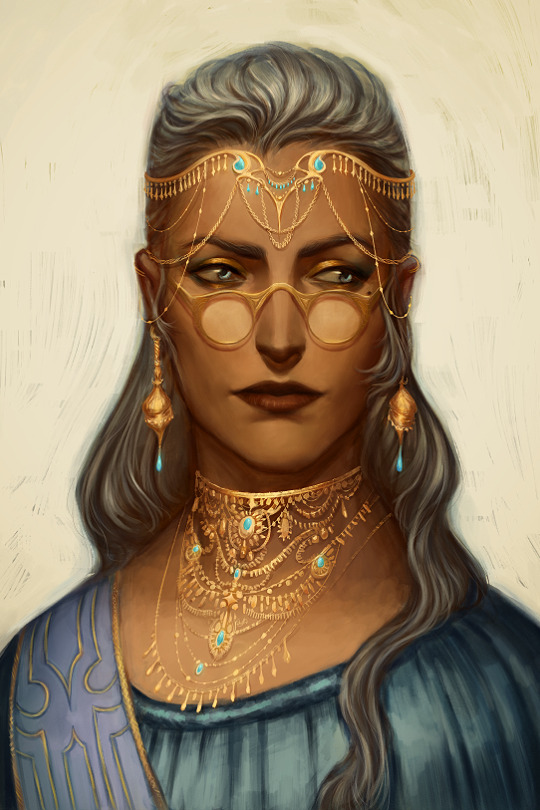
\includegraphics[width=.55\textwidth]{./resources/Favilla}
  \caption{
    Favilla, Opi's lover.
  }
\end{figure}

\section{Backstory}

{\it To be read in the context of Opi as the narrator.}

\noindent
Once, long ago, I was a blacksmith in small village of Nilfgaard. I was talented, or atleast
I considered myself so. You see, I rarely ventured out of my house, let alone out of town. I never
knew how I stacked up, though the villagers seemed perfectly content to trade food and ores for the
occasional metalworking job. I reckon they were just happy to save their coin, but I didn't want for
much. There was an endless world of complexity in my craft to lose myself in. Immersed, my whiskers
eventually grew gray, and I bet they would've eventually grown dead if she hadn't shown up.

{\it Favilla}. Before my door, she stood, tall in stature and presense. She presented me with
a small sword; I recognized it, seems long ago I had been contracted to make a few swords, probably
for some army for some war.


Once, long ago, I was an ordinary blacksmith in a small village of Nilfgaard.

Walking through the poorly lit streets of Waterdeep, the cloaked man, having
seemingly appeared out of nowhere, coughed into his hand. Clenching his fist,
blood streamed off of his knuckles and dripped onto the pavement. He was dying.
But he was certain that the poison wouldn't take him immediately. It wasn't in
their nature to afford him a clean death. Dimly, he wondered if he should be
grateful for their sadism that allowed him to live until this point.

He glanced down to his sword, which glew with the light of the {\em locate
creature} spell he had been maintaining. The spectral trail emanating from the
blade, which passerbys strangely seemed to be unaware of, had stopped at the
enterance of a tavern. {\em The Adventurer's Respite}. His fine elven nose
turned up at the smell. Gritting his teeth, however, he walked in.

His eyes brightened upon entering, ignoring the smashed patrons and instead focusing
on an half-elven figure behind the counter. The {\em locate creature} spell,
with the completion of its task, faded, and the elven man waded through the
patrons to stand by the counter. He glanced at her, and was dazed for a moment.
She looked just like her... but then he grimaced.

Merely an half-elf, her lifespan was already nearing its end. She was too old,
he could see her fingers slightly tremble with age, her footsteps loud,
revealing the weakness in his bones, her body. He wanted to laugh bitterly, but
could only cough. This time the blood was tinged with black. He knew he didn't
have long. Seeing her walk over in concern, he shook away his lethargy and asked
her 'Do you have any descendents?' 

The unfriendly look in her eyes told him all he needed to know. He sighed,
knowing he had no other option than this poor one. There were none left. Slowly,
he reached for his blade, unclipped it, and placed it heavily onto the counter.
He looked into her shocked eyes, and gravely said 'Descendent of the Song,
I leave this in your care. Protect yourself well.' And with that, as his hand
left the blade his form shifted and dispersed into a cloud of nothingness.

Later that night, Song Xia, sat in her room above {\em The Adventurer's Respite}
and stared at the blade with a strange look in her eyes. When the man had
dispersed earlier in the day, she had cried out in fear. But strangely, not
a single other person in the bar had reacted to the spectacle, and she had to
embarrassedly apologize to the tavern. It's as if no one else had seen that man.
Looking down at the blade, she saw intricate runes engraved across the blade,
but she couldn't understand them. She had forgotten all of the Elven taught to
her in her youth. Unconsciously, she reached out a hand to touch them, and when
she did a name floated into her mind. {\em Ghaunavel}. She didn't even have time
to scream before the blue arcane fires of the blade-rite enveloped her.

\end{document}
